\section{Technologie}
	\subsection{Server}

		\subsubsection{Evaluation}\label{serverEvaluation}
			Die Servertechnologie stellt eine entscheidende Komponente dar, 
			ihre Wahl ist von entschprechender Tragweite für andere Komponenten des Projektes.
			Aus diesem Grund haben wir sie ausführlich evaluiert.
			
			\begin{enumerate}
				\item Schritt: Gemeinsame Definition von Kriterien und möglichen Servertechnologien.
				\item Schritt: Sepparate Festlegung der Gewichtung der Kriterien sowie Definition der Matrix Kriterium/Servertechnologie mit der persönliche Schätzung, wie stark jede Servertechnologie das entsprechende Kriterium erfüllt.
				\item Schritt: Zusammenführung der persönlichen Ergebnisse zu Gesammtergebnis
			\end{enumerate}
		
			\begin{figure}[H]
				\begin{minipage}[b]{\linewidth}
					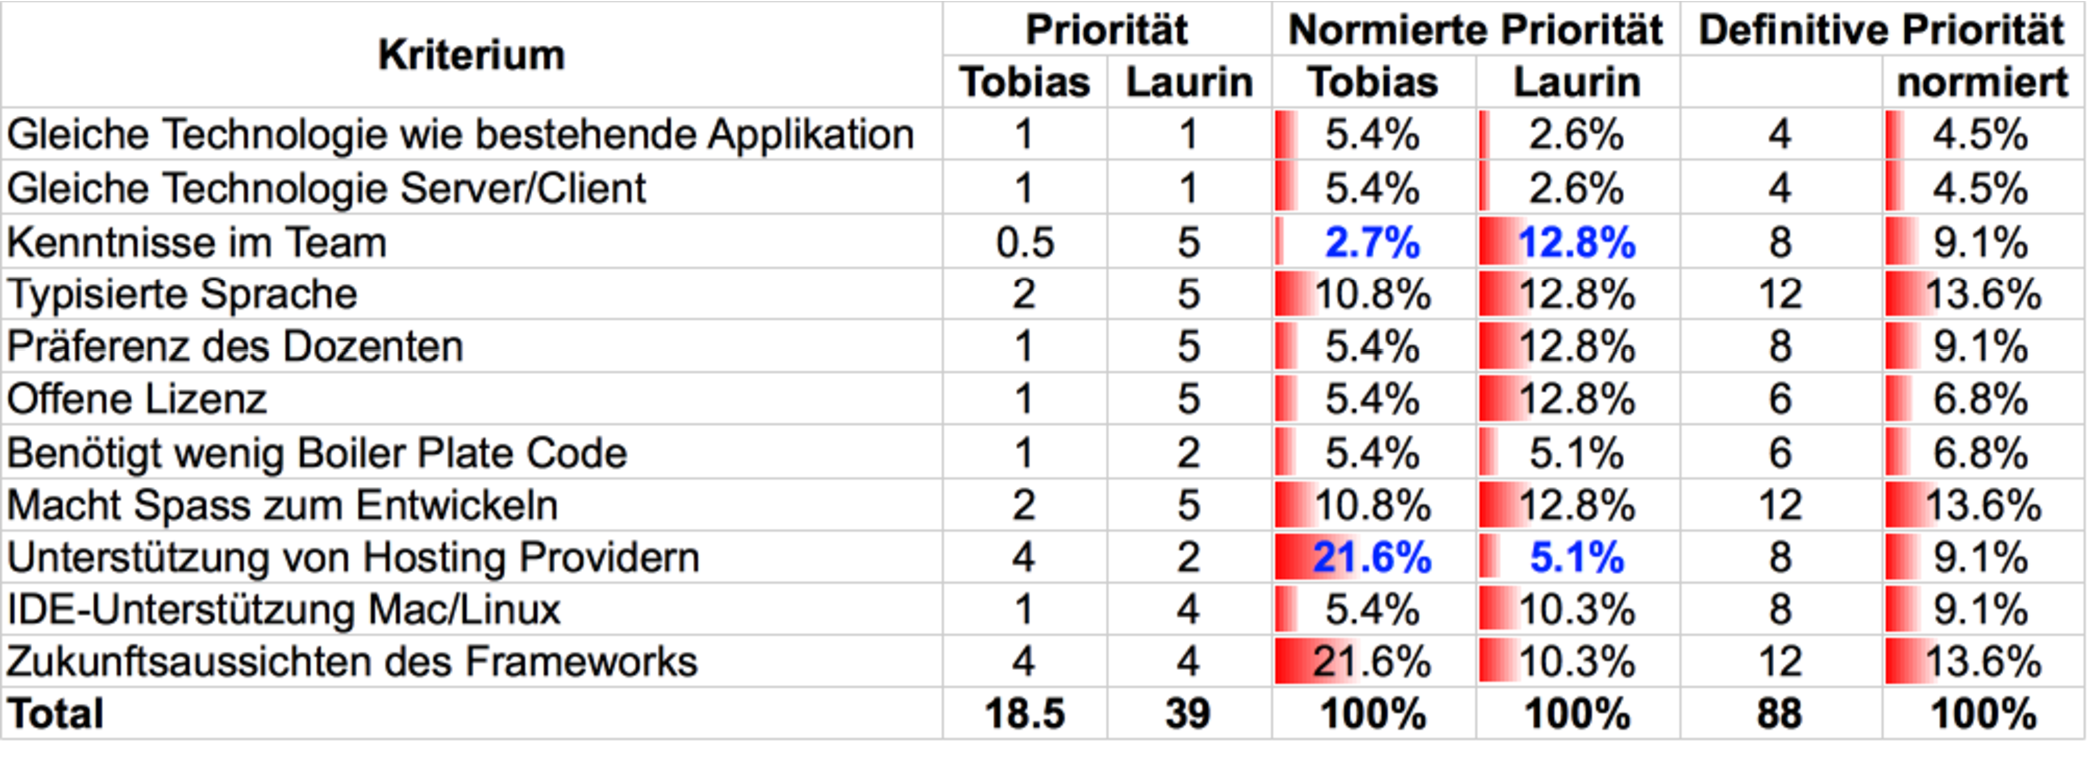
\includegraphics[width=\textwidth]{media/spreadsheets/ServertechnologieVergleichPrioritaetsfinding.pdf}
					\centering
					\caption{Servertechnologie-Vergleich: Prioritätsfinding}
					\label{fig:ServertechnologieVergleichPrioritaetsfinding}
				\end{minipage}
			\end{figure}
			
			Abbildung~\ref{fig:ServertechnologieVergleichPrioritaetsfinding} zeigt den Prozess der Prioritätsfindung.
			Wie bereits erwähnt, haben wir zuerst die Kriterien definiert und 
			anschliessend je separat Prioritäten für jedes Kriterium festgelegt.
			Da wir verschiedene Skalen verwendet haben, haben wir unsere Punkte noch zu 100\% normiert.
			Und aus diesen zwei Werten haben wir in gemeinsamer Diskussion die definitive Priorität erstellt.
			Dies hat meist problemlos funktioniert, ausser bei den Punkten "`Kenntnisse im Team"' und "`Unterstützung von Hosting Providern"' (blau markiert) hatten wir zu Beginn nennenswerte Unterschiede.
			Bei diesen Punkten haben wir dann in der gemeinsamen Diskussion einen Wert festgelegt.
		
			\begin{figure}[H]
				\begin{minipage}[b]{\linewidth}
					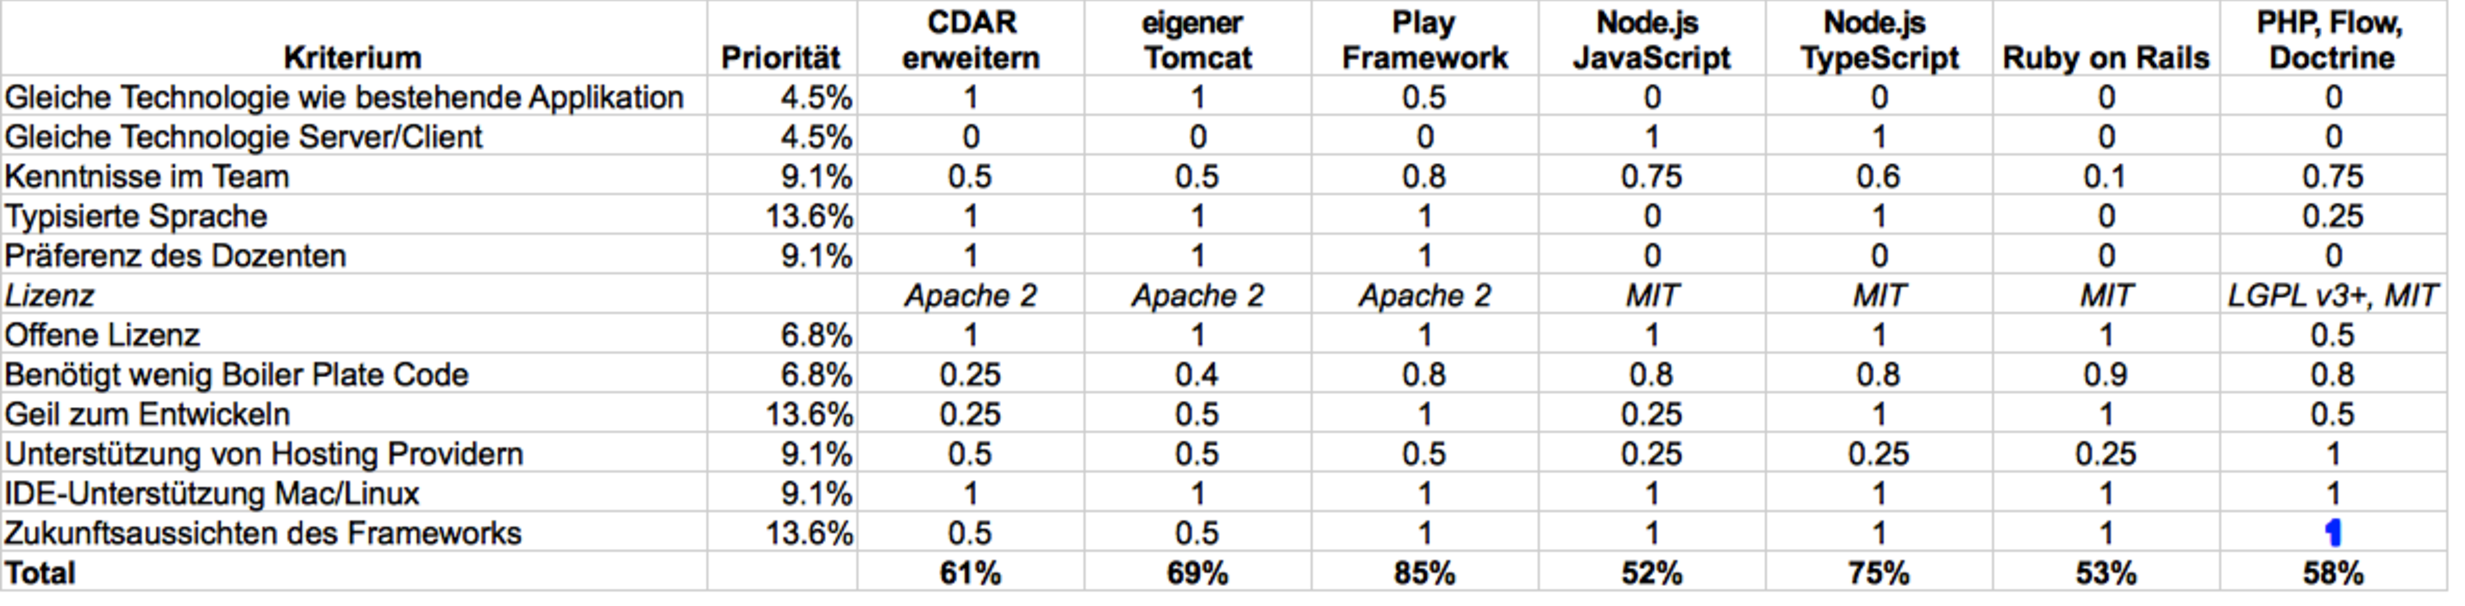
\includegraphics[width=\textwidth]{media/spreadsheets/ServertechnologieVergleichVergleichDerTechnologien.pdf}
					\centering
					\caption{Servertechnologie-Vergleich: Vergleich der Technologien}
					\label{fig:ServertechnologieVergleichVergleichDerTechnologien.pdf}
				\end{minipage}
			\end{figure}
			
			Abbildung~\ref{fig:ServertechnologieVergleichVergleichDerTechnologien.pdf} zeigt den Vergleich der einzeln evaluierten Servertechnologien.
			Auch hier haben wir zuerst je separat die Schätzung gemacht und dann verglichen.
			Bei diesem Vergleich haben wir gar noch ähnlichere Werte gewählt, lediglich bei den Zukunftsaussichten von PHP, Flow und Doctrine (blau markiert) hatten wir nennenswert unterschiedliche Ansichten.
			
			\begin{figure}
					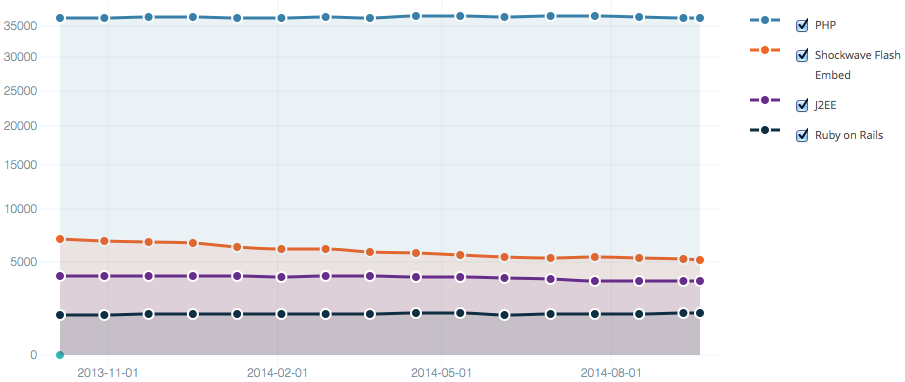
\includegraphics[width=\textwidth]{media/img/EntwicklungVonWebserverTechnologien.png}
					\centering
					\caption{Entwicklung von Webserver"=Technologien der Top 10'000 Sites \cite{sharesOfWebtechnologies}}
					\label{fig:EntwicklungVonWebserverTechnologien}
			\end{figure}
			
			Schlussendlich haben wir uns da nach Recherchen auf eine "`1"' geeinigt, weil entgegen den Erwartungen von Laurin Murer sich die Verbreitung von PHP (auch von den grösseren Seiten) kaum verändert hat.
			Als Beispiel für eine Technologie die am aussterben ist haben wir Shockwave Flash herangezogen, welche, wie in Abbildung~\ref{fig:EntwicklungVonWebserverTechnologien} sichtbar, im letzten Jahr deutlich an Boden verloren hat.
			Im Vergleich dazu ist PHP sehr gut im Markt vertreten und hat auch eine äusserst konstante Verbreitung.
			Deshalb und unter dem Gesichtspunkt von jungen modernen PHP Frameworks wie Doctrine und Flow sehen wir da auch die Zukunftsaussichten gegeben.
			
			\begin{figure}[H]
				\begin{minipage}[b]{\linewidth}
					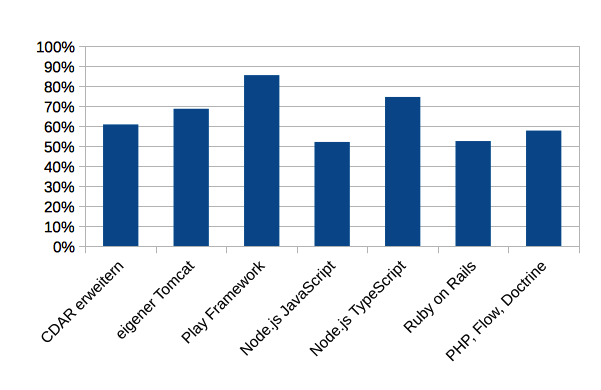
\includegraphics[width=\textwidth]{media/spreadsheets/ServertechnologieVergleichVergleichDerTechnologienDiagramm.png}
					\centering
					\caption{Ergebnis Servertechnologie-Vergleich}
					\label{fig:ErgebnisServertechnologieVergleich}
				\end{minipage}
			\end{figure}
			
			Schlussendlich haben wir für jede Technologie das Total der Punkte berechnet (Punkte jedes Kriteriums multipliziert mit seiner Priorität). in Abbildung~\ref{fig:ErgebnisServertechnologieVergleich} zeigt man das finale Ergebnis. Aufgrund diesem haben wir uns für das Play Framework entschieden. Eine Alternative wäre noch Node.js mit TypeScript gewesen, doch dies hat bereits 10\%-Punkte weniger erreicht.

		\subsubsection{Play Framework}
			Kapitel~\ref{serverEvaluation} erläutert den Hintergrund der Entscheidung für das Play Framework. 
			Wikipedia beschreibt das Play Framework wie folgt:
			\begin{quote}
				"`Play is an open source web application framework, written in Scala and Java, which follows the model–view–controller (MVC) architectural pattern. It aims to optimize developer productivity by using convention over configuration, hot code reloading and display of errors in the browser."'\cite{playFrameworkWikipedia}
			\end{quote}
			
			
			Zusammenfassend führten die folgenden Gründe zur Entscheidung für das Play Framework:
			\begin{itemize}
				\item Das Play Framework basiert auch auf Java, wie das bestehende CDAR.
				\item Ein Teammitglied hat bereits Erfahrungen mit dem Framework gemacht.
				\item Das andere Teammitglied kennt die zugrundeliegende Sprache (Java).
				\item Der betreuende Dozent hat eine Präferenz für Java.
				\item Das Play Framework benötigt wenig Boilerplate-Code.
				\item Es sprechen keine zwingenden Gründe dagegen (wie beispielsweise zu stark einschränkende Lizenzen).
				\item Das Play Framework ist angenehm zum Entwickeln für die Entwickler: gegebener Spass-Faktor, Vermeidung von Fehlern, Unterstützung im Erreichen von guter Code Qualität.
			\end{itemize}

			

	\subsection{Client}
		\subsubsection{Sprache}
			\begin{tabularx}{\textwidth}{|lXX|}
				\hline
					\textbf{} & \textbf{Vorteile} & \textbf{Nachteile}\\
				\hline
					\textbf{JavaScript} & 
					\begin{itemize}
						\item UI der bestehenden Applikation ist auch in JavaSscript geschrieben
					\end{itemize} & 
					\begin{itemize}
						\item Fehler tauchen erst zur Runtime auf
						\item Sprachspezifische Besonderheiten, die Fehler begünstigen
					\end{itemize} \\
				\hline
					\textbf{TypeScript} &
					\begin{itemize}
						\item Wird kompiliert (zu Javascript), weniger Fehler zur Runtime
						\item Optisch besser lesbar als JavaScript
					\end{itemize} &
					\begin{itemize}
						\item Erfordert TSC-Compiler
						\item Code Overhead bei Inheritance
					\end{itemize} \\
				\hline
			\end{tabularx}
			
			
		\subsubsection{Architektur-Framework}
			\begin{tabularx}{\textwidth}{|lXX|}
				\hline
					\textbf{} & \textbf{Vorteile} & \textbf{Nachteile}\\
				\hline
					\textbf{Angular JS} &
					\begin{itemize}
						\item bekanntes MVW- und Templating Framework, erlaubt eine saubere Trennung von Logik und Darstellung
						\item bindet ViewModel Properties und Functions ans Template, wodurch sich Observerkonstrukte sparen lassen
						\item ist stabil, zuverlässig, gut erweiterbar und bringt von sich aus schon sehr viel mit
						\item wurde auch schon für die bestehende Applikation eingesetzt
					\end{itemize} &
					\begin{itemize}
						\item Attribute Binding besitzt gewissen Overhead
					\end{itemize} \\
				\hline
					\textbf{Ember JS} &				
					\begin{itemize}
						\item Sehr Modular und anpassbar
						\item Weniger Overhead als AngularJS
					\end{itemize} &
					\begin{itemize}
						\item Bringt wesentlich weniger mit als Angular JS, mehr Eigenaufwand notwendig
					\end{itemize} \\
				\hline
					\textbf{Kein Framework} &
					\begin{itemize}
						\item Vollständig freie Architekturgestaltung
					\end{itemize} &
					\begin{itemize}
						\item Hoher Implementationsaufwand ohne Gewinn
					\end{itemize} \\
				\hline
			\end{tabularx}
			
			\subsubsection{Require.js}
				Require.js eignet sich gut zur Strukturierung und zum Autolading der Klassen und komponenten, 
				insbesondere während der Entwicklung.

		\subsection{UI Frameworks}
			\subsubsection{LESS}
				Less soll als CSS Generator eingesetzt werden, da es den CSS Code stark verschlankt und Vorteile wie Variablen und Mixins bietet. LESS kann bei einem Node.js Server serverseitig compiled werden um den Client zu entlasten.
				
		\subsection{Testing}
			Testing Framework Anforderungen:
			\begin{itemize}
				\item Einfach einzubinden
				\item Einfach zu erweitern
				\item Bekannte Benutzung mit Tests und Asserts
				\item Möglichkeit zur Anbindung eines Build Tools
			\end{itemize}

			\subsubsection{JsUnit / QUnit}
				JsUnit wie QUnit arbeiten mit einem realen Browser (keine Browsersimulation), 
				sind einfach handzuhaben und bieten typische Assert-Syntax.
				
				
